\documentclass[12pt]{article}
\usepackage{graphicx}			    % Use this package to include images %Path relative to the main .tex file 
\graphicspath{ {./Images/} }
\usepackage{amsmath}			    % A library of many standard math expressions
\usepackage{mathtools}              % For Aboxed{} (https://tex.stackexchange.com/questions/346577/boxed-and-align)
% \usepackage[margin=1in]{geometry} % Sets 1in margins. 
\usepackage[margin=2.5cm]{geometry} % Sets 1in margins. 
\usepackage{fancyhdr}			    % Creates headers and footers
\usepackage{enumerate}              % These two packages give custom labels to a list
\usepackage[shortlabels]{enumitem}
\usepackage{hyperref}               % https://www.overleaf.com/learn/latex/Hyperlinks
\usepackage{xcolor}
\usepackage[svgnames]{xcolor}
\usepackage{float}
\usepackage{cmupint}                % For upright integrals. https://tex.stackexchange.com/questions/503527/how-to-write-upright-integrals-with-automatic-sizing
\usepackage{tikz}
\usetikzlibrary{trees, graphs}
\usetikzlibrary{calc, shapes.multipart, chains, arrows}
\usetikzlibrary{arrows.meta, positioning}
\usepackage{titling}
\usepackage{minted}                 % For code blocks
\usemintedstyle{monokai}            % For code blocks
\definecolor{bg}{HTML}{282828}      % For code blocks, from https://github.com/kevinsawicki/monokai
\usepackage{nameref}
\usepackage{caption}                % To use \caption*{} to show only the caption text without "Table 1: <text>"
\usepackage{multicol}
% \usepackage{mathtools, tccomicsans}
% \usepackage{comicsans}
% \usepackage[main,largesymbols]{tccomicsans} % https://www.reddit.com/r/LaTeX/comments/1l5no5d/comment/mwm64ze/
\renewcommand*\contentsname{Summary}
% \renewcommand{\contentsname}{\centering \normalfont\normalsize Contents}
\renewcommand{\contentsname}{\centering \bfseries\Large Contents}
% \renewcommand{\cftaftertoctitle}{\hfill}

\hypersetup
{
    colorlinks=true,
    linkcolor=blue,
    filecolor=magenta,      
    urlcolor=cyan,
    %pdftitle={Overleaf Example},
    pdfpagemode=FullScreen,
}

% \title{OOP Lab Manual 05}
% \author{STM}
% \date{December 2024}

\begin{document}

\begin{titlepage}
    \centering

    \vspace*{-4em}
    \includegraphics[width=0.5\textwidth]{Bismillah.png}%\\[2cm]
    \vspace*{5em}

    
    \vspace*{1cm}

     \includegraphics[width=0.5\textwidth]{GU Tech 1685x1330.png}\\[2cm]

    \MakeUppercase{\Huge \textbf{GU TECH}}\\[1.5ex]
    
    \vspace*{1cm}
    
    \Huge Data Structures \\[1.5ex]
    \LARGE Lab 12 \\[2cm]

    % {\Large STM} \\ [2cm]

    {\Large \today}\\[1cm]
    
\end{titlepage}

\newpage

% \vspace*{4cm}
% \begin{center}
%     \Huge \textbf{Outline}
% \end{center}

% \begin{itemize}
%    \item \nameref{Functions}
% \end{itemize}

\tableofcontents

























\newpage
\addcontentsline{toc}{part}{Lab Tasks}
\part*{\centering Lab Tasks}

\begin{enumerate}

    \item Implement a \textcolor{red}{\texttt{Graph}} class using both adjacency matrix and adjacency list representations, and implement the following:
    \begin{itemize}
        \item Warshall's algorithm for accessibility.
        \item Floyd's all pairs shortest path algorithm with \textbf{path tracking}.
        \begin{itemize}
            \item Your code should contain a function that takes the two output matrices and any two nodes, and prints the shortest path between them if there is any. 
        \end{itemize}
        \item Dijkstra's single source shortest path algorithm.
        \begin{itemize}
            \item Your code should contain a function that takes the output of Dijkstra's algorithm and any two nodes, and prints the shortest path between them if there is any.
        \end{itemize}
        \item BFS based single source shortest path algorithm.
        \item Prim's and Kruskal's algorithms for minimum spanning tree.
    \end{itemize}

    \textbf{Requirements:}
    \begin{itemize}
        \item Users should be able to select the representation (adjacency matrix or adjacency list) at the time of object creation.
        \item Users should not be required to provide names of nodes. If no names are provided, the class should assign single letter names starting from `A' until `Z', at least for the first 26 nodes.
    \end{itemize}

    \textbf{Instructions:}

    \begin{itemize}
        \item There is no starter code.
        \item Algorithm functions do not necesarily need to be members of a class.
        \item Submit screenshots of the test cases along with your code files.
    \end{itemize}





    \newpage
    \textbf{Testing:}

    \begin{itemize}
        \item For Floyd Warshall algorithm, use the given graph. Your distance and predecessor matrices should be:
    
        \begin{multicols}{2}
        
    \begin{table}[H]
        \makebox[\linewidth][c]
        {
            \begin{tabular}{| c | c | c | c |} 
                \hline
                0 & 2 & 4 & 3 \\
                \hline
                3 & 0 & 2 & 6 \\
                \hline
                2 & 4 & 0 & 4 \\
                \hline
                -2 & 0 & 2 & 0 \\
                \hline
            \end{tabular}
        }
        % \caption*{}
    \end{table}

    \begin{table}[H]
        \makebox[\linewidth][c]
        {
            \begin{tabular}{| c | c | c | c |} 
                \hline
                - & A & B & A \\
                \hline
                B & - & B & A \\
                \hline
                D & A & - & C \\
                \hline
                D & A & B & - \\
                \hline
            \end{tabular}
        }
        % \caption*{}
    \end{table}

            % \textcolor{red}{\texttt{0, 2, 4, 3}} \\
            % \textcolor{red}{\texttt{3, 0, 2, 6}} \\
            % \textcolor{red}{\texttt{2, 4, 0, 4}} \\
            % \textcolor{red}{\texttt{-2, 0, 2, 0}} \\
                
            % \textcolor{red}{\texttt{-, A, B, A}} \\
            % \textcolor{red}{\texttt{B, -, B, A}} \\
            % \textcolor{red}{\texttt{D, A, -, C}} \\
            % \textcolor{red}{\texttt{D, A, B, -}} \\

    \end{multicols}

    As such, the path from \textcolor{red}{\texttt{C}} to \textcolor{red}{\texttt{B}}, for example, should be: \textcolor{red}{\texttt{C -> D -> A -> B}}.    
    

    \begin{figure}[H]
        \centering
        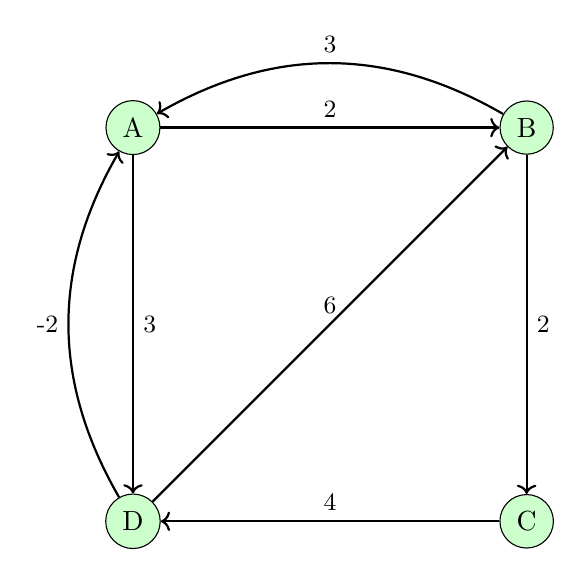
\begin{tikzpicture}[
            node/.style={circle, draw, fill=green!20, minimum size=18pt},
            edge/.style={->, thick},
            weight/.style={font=\small, midway}
        ]

        % Nodes (manual layout to match figure)
        \node[node] (A) at (0, 5) {A};
        \node[node] (B) at (5, 5) {B};
        \node[node] (C) at (5, 0) {C};
        \node[node] (D) at (0, 0) {D};

        % Edges

        \draw[edge] (A) -- node[weight, above] {2} (B);
        \draw[edge] (A) -- node[weight, right] {3} (D);

        \draw[edge, bend left=-30] (B) to node[weight, above] {3} (A);
        \draw[edge] (B) -- node[weight, right] {2} (C);

        \draw[edge] (C) -- node[weight, above] {4} (D);

        \draw[edge, bend left=30] (D) to node[weight, left] {-2} (A);
        \draw[edge] (D) -- node[weight, above] {6} (B);

        \end{tikzpicture}
    \caption{Directed graph for testing Floyd-Warshall algorithm}
    \end{figure}

    \begin{center}
        \href{https://www.youtube.com/watch?v=sLg6Leb-xt0}{Graph source}
    \end{center}

    \newpage
    \item For Dijkstra's algorithm, use the given graph and return the following output matrix (assuming that the source node is \textcolor{red}{\texttt{A}}):
    
    \begin{table}[H]
        \makebox[\linewidth][c]
        {
            \begin{tabular}{| c | c | c |} 
                \hline
                \textbf{Node} & \textbf{Shortest Distance} & \textbf{Previous Node} \\ [1ex]
                \hline
                A & 0 &  \\	
                \hline
                B & 2 & A \\
                \hline
                C & 12 & F \\
                \hline
                D & 7 & B \\
                \hline
                E & 8 & B \\
                \hline
                F & 9 & D \\
                \hline
            \end{tabular}
        }
        % \caption*{}
    \end{table}

    As such, the path from \textcolor{red}{\texttt{A}} to \textcolor{red}{\texttt{C}}, for example, should be: \textcolor{red}{\texttt{A -> B -> D -> F -> C}} for a cost of 12 units.

    \textbf{Note:} Your output does not necessarily need to be a $3 \times 1$ matrix. You are free to format your output in any way you like, as long as it contains the required information. 

    \begin{figure}[H]
        \centering
        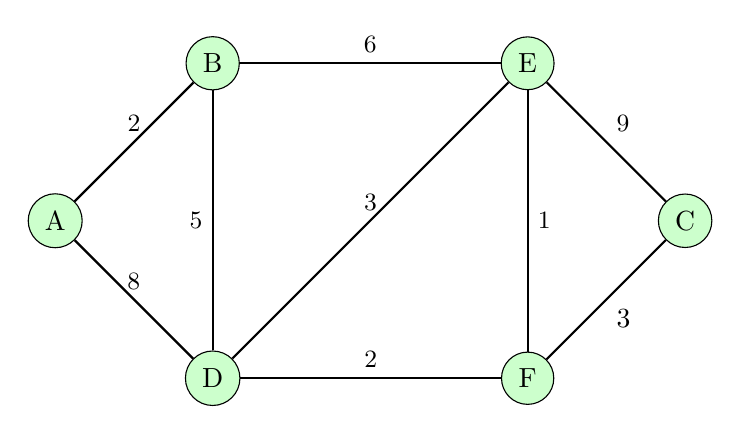
\begin{tikzpicture}[
            node/.style={circle, draw, fill=green!20, minimum size=18pt},
            edge/.style={-, thick},
            weight/.style={font=\small, midway}
        ]

        % Nodes (manual layout to match figure)
        \node[node] (A) at (-4, 0) {A};
        \node[node] (B) at (-2, 2) {B};
        \node[node] (C) at (4, 0) {C};
        \node[node] (D) at (-2, -2) {D};
        \node[node] (E) at (2, 2) {E};
        \node[node] (F) at (2, -2) {F};

        % Edges
        % \draw[edge, bend left=-30] (B) to node[weight, above] {3} (A);

        \draw[edge] (A) -- node[weight, above] {2} (B);
        \draw[edge] (A) -- node[weight, above] {8} (D);

        \draw[edge] (B) -- node[weight, left] {5} (D);
        \draw[edge] (B) -- node[weight, above] {6} (E);

        \draw[edge] (C) -- node[weight, above right] {9} (E);
        \draw[edge] (C) -- node[below right] {3} (F);

        \draw[edge] (D) -- node[weight, above] {3} (E);
        \draw[edge] (D) -- node[weight, above] {2} (F);

        \draw[edge] (E) -- node[weight, right] {1} (F);

    \end{tikzpicture}
    \caption{Undirected graph for testing Dijkstra's algorithm}
    \end{figure}

    \begin{center}
        \href{https://www.youtube.com/watch?v=bZkzH5x0SKU}{Graph source}
    \end{center}













    \newpage
    \item For Prim's algorithm, use the given graph and return the following output matrix (assuming that the source node is \textcolor{red}{\texttt{A}}):

    \begin{table}[H]
        \makebox[\linewidth][c]
        {
            \begin{tabular}{| c | c |} 
                \hline
                \textbf{Edge} & \textbf{Weight Distance} \\ [1ex]
                \hline
                A - B & 2 \\ 
                \hline
                A - C & 3 \\ 
                \hline
                A - D & 3 \\ 
                \hline
                C - E & 1 \\ 
                \hline
                C - F & 6 \\ 
                \hline
                F - G & 9 \\ 
                \hline
            \end{tabular}
        }
        % \caption*{}
    \end{table}

    \begin{figure}[H]
        \centering
        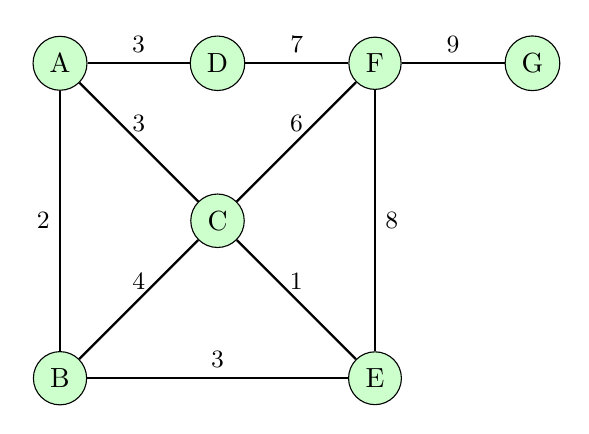
\begin{tikzpicture}[
            node/.style={circle, draw, fill=green!20, minimum size=18pt},
            edge/.style={-, thick},
            weight/.style={font=\small, midway}
        ]

        % Nodes (manual layout to match figure)
        \node[node] (A) at (-2, 2) {A};
        \node[node] (B) at (-2, -2) {B};
        \node[node] (C) at (0, 0) {C};
        \node[node] (D) at (0, 2) {D};
        \node[node] (E) at (2, -2) {E};
        \node[node] (F) at (2, 2) {F};
        \node[node] (G) at (4, 2) {G};

        % Edges
        % \draw[edge, bend left=-30] (B) to node[weight, above] {3} (A);

        \draw[edge] (A) -- node[weight, left] {2} (B);
        \draw[edge] (A) -- node[weight, above] {3} (C);
        \draw[edge] (A) -- node[weight, above] {3} (D);

        \draw[edge] (B) -- node[weight, above] {4} (C);
        \draw[edge] (B) -- node[weight, above] {3} (E);

        \draw[edge] (C) -- node[weight, above] {1} (E);
        \draw[edge] (C) -- node[weight, above] {6} (F);

        \draw[edge] (D) -- node[weight, above] {7} (F);

        \draw[edge] (E) -- node[weight, right] {8} (F);

        \draw[edge] (F) -- node[weight, above] {9} (G);

    \end{tikzpicture}
    \caption{Undirected graph for testing Prim's algorithm}
    \end{figure}

    \begin{center}
        \href{https://youtu.be/cplfcGZmX7I}{Graph source}
    \end{center}

    \begin{figure}[H]
        \centering
        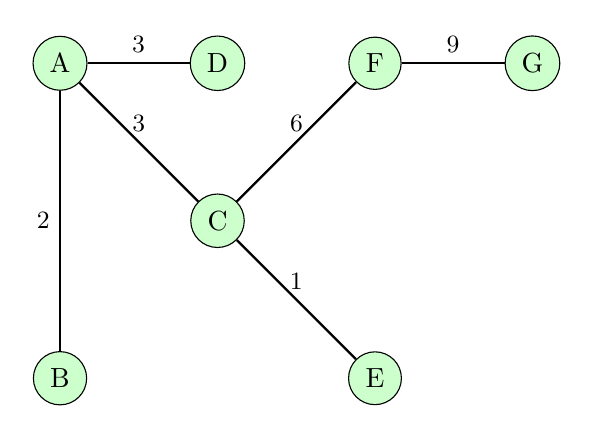
\begin{tikzpicture}[
            node/.style={circle, draw, fill=green!20, minimum size=18pt},
            edge/.style={-, thick},
            weight/.style={font=\small, midway}
        ]

        % Nodes (manual layout to match figure)
        \node[node] (A) at (-2, 2) {A};
        \node[node] (B) at (-2, -2) {B};
        \node[node] (C) at (0, 0) {C};
        \node[node] (D) at (0, 2) {D};
        \node[node] (E) at (2, -2) {E};
        \node[node] (F) at (2, 2) {F};
        \node[node] (G) at (4, 2) {G};

        % Edges
        % \draw[edge, bend left=-30] (B) to node[weight, above] {3} (A);

        \draw[edge] (A) -- node[weight, left] {2} (B);
        \draw[edge] (A) -- node[weight, above] {3} (C);
        \draw[edge] (A) -- node[weight, above] {3} (D);

        \draw[edge] (C) -- node[weight, above] {1} (E);
        \draw[edge] (C) -- node[weight, above] {6} (F);

        \draw[edge] (F) -- node[weight, above] {9} (G);

    \end{tikzpicture}
    \caption{MST by Prim's algorithm for the given graph}
    \end{figure}









    \newpage
    \item For Kruskal's algorithm, use the given graph and return the following output matrix (assuming that the source node is \textcolor{red}{\texttt{A}}):

    \begin{table}[H]
        \makebox[\linewidth][c]
        {
            \begin{tabular}{| c | c |} 
                \hline
                \textbf{Edge} & \textbf{Weight Distance} \\ [1ex]
                \hline
                A - B & 2 \\ 
                \hline
                A - C & 3 \\ 
                \hline
                A - D & 3 \\ 
                \hline
                C - E & 1 \\ 
                \hline
                D - F & 7 \\ 
                \hline
                F - G & 9 \\ 
                \hline
            \end{tabular}
        }
        % \caption*{}
    \end{table}

    \begin{figure}[H]
        \centering
        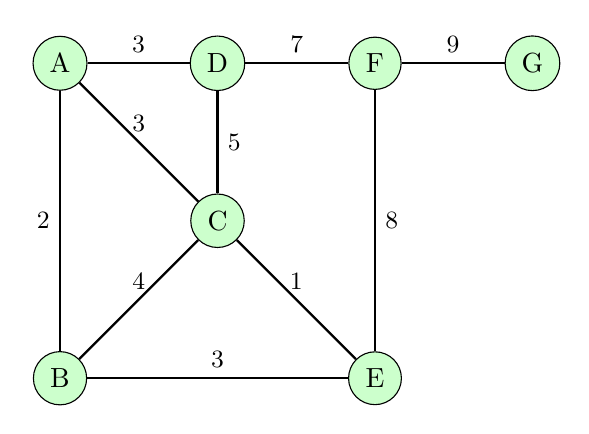
\begin{tikzpicture}[
            node/.style={circle, draw, fill=green!20, minimum size=18pt},
            edge/.style={-, thick},
            weight/.style={font=\small, midway}
        ]

        % Nodes (manual layout to match figure)
        \node[node] (A) at (-2, 2) {A};
        \node[node] (B) at (-2, -2) {B};
        \node[node] (C) at (0, 0) {C};
        \node[node] (D) at (0, 2) {D};
        \node[node] (E) at (2, -2) {E};
        \node[node] (F) at (2, 2) {F};
        \node[node] (G) at (4, 2) {G};

        % Edges
        % \draw[edge, bend left=-30] (B) to node[weight, above] {3} (A);

        \draw[edge] (A) -- node[weight, left] {2} (B);
        \draw[edge] (A) -- node[weight, above] {3} (C);
        \draw[edge] (A) -- node[weight, above] {3} (D);

        \draw[edge] (B) -- node[weight, above] {4} (C);
        \draw[edge] (B) -- node[weight, above] {3} (E);

        \draw[edge] (C) -- node[weight, right] {5} (D);
        \draw[edge] (C) -- node[weight, above] {1} (E);

        \draw[edge] (D) -- node[weight, above] {7} (F);

        \draw[edge] (E) -- node[weight, right] {8} (F);

        \draw[edge] (F) -- node[weight, above] {9} (G);

    \end{tikzpicture}
    \caption{Undirected graph for testing Kruskal's algorithm}
    \end{figure}

    \begin{center}
        \href{https://www.youtube.com/watch?v=71UQH7Pr9kU}{Graph source}
    \end{center}

    \begin{figure}[H]
        \centering
        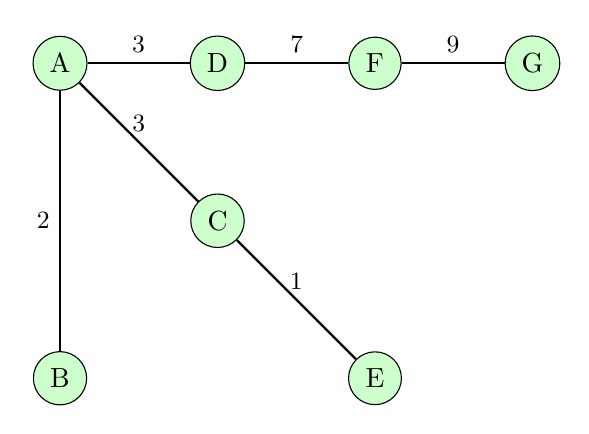
\begin{tikzpicture}[
            node/.style={circle, draw, fill=green!20, minimum size=18pt},
            edge/.style={-, thick},
            weight/.style={font=\small, midway}
        ]

        % Nodes (manual layout to match figure)
        \node[node] (A) at (-2, 2) {A};
        \node[node] (B) at (-2, -2) {B};
        \node[node] (C) at (0, 0) {C};
        \node[node] (D) at (0, 2) {D};
        \node[node] (E) at (2, -2) {E};
        \node[node] (F) at (2, 2) {F};
        \node[node] (G) at (4, 2) {G};

        % Edges
        % \draw[edge, bend left=-30] (B) to node[weight, above] {3} (A);

        \draw[edge] (A) -- node[weight, left] {2} (B);
        \draw[edge] (A) -- node[weight, above] {3} (C);
        \draw[edge] (A) -- node[weight, above] {3} (D);

        \draw[edge] (C) -- node[weight, above] {1} (E);

        \draw[edge] (D) -- node[weight, above] {7} (F);

        \draw[edge] (F) -- node[weight, above] {9} (G);

    \end{tikzpicture}
    \caption{MST by Kruskal's algorithm for the given graph}
    \end{figure}













    \end{itemize}











    % \begin{figure}[h]
    %     \centering
    %     \begin{tikzpicture}[
    %         node/.style={circle, draw, fill=green!20, minimum size=18pt},
    %         edge/.style={->, thick},
    %         weight/.style={font=\small, midway}
    %     ]

    %     % Nodes (manual layout to match figure)
    %     \node[node] (0) at (0,2) {0};
    %     \node[node] (1) at (3,2) {1};
    %     \node[node] (2) at (-1,0) {2};
    %     \node[node] (3) at (1,0) {3};
    %     \node[node] (4) at (4,0) {4};

    %     % Edges
    %     \draw[edge] (0) -- node[weight, above] {4} (1);
    %     \draw[edge] (0) -- node[weight, right] {5} (3);

    %     % \draw[edge, bend left=25] (1) -- node[weight, above] {1} (2);
    %     \draw[edge, bend left=15] (1) to node[weight, above] {1} (2);
    %     \draw[edge] (1) -- node[weight, right] {6} (4);

    %     \draw[edge] (2) -- node[weight, right] {2} (0);
    %     \draw[edge] (2) -- node[weight, below] {3} (3);

    %     \draw[edge, bend left=45] (3) to node[weight, below] {1} (2);
    %     \draw[edge] (3) -- node[weight, below] {2} (4);

    %     \draw[edge, bend left=45] (4) to node[weight, below] {4} (3);
    %     \draw[edge] (4) -- node[weight, below right] {1} (0);

    %     \end{tikzpicture}
    % \end{figure}

    % \begin{figure}[h]
    % \centering
    % \begin{tikzpicture}[
    %     vertex/.style={circle, draw, minimum size=8mm},
    %     edge/.style={->, >=Stealth, thick}
    % ]

    % % Arrange nodes in a circle
    % \foreach \i/\angle/\label in {0/0/0,1/60/1,2/120/2,3/180/3,4/240/4,5/300/5,6/360/6}
    % {
    %     \node[vertex] (\label) at (\angle:3) {\label};
    % }

    % % Draw unique edges only
    % \draw[edge] (1) -- (0);
    % \draw[edge] (0) -- (4);
    % \draw[edge] (1) -- (2);
    % \draw[edge] (2) -- (6);
    % \draw[edge] (6) -- (5);
    % \draw[edge] (2) -- (3);
    % \draw[edge] (3) -- (4);
    % \draw[edge] (4) -- (3);

    % \end{tikzpicture}
    % \caption{Simple directed graph}
    % \label{fig:simple-graph}
    % \end{figure}

    % \begin{figure}[h]
    % \centering
    % \begin{tikzpicture}[
    %     node distance=2.5cm,
    %     vertex/.style={circle, draw, minimum size=8mm, font=\sffamily\large},
    %     arrow/.style={->, >=Stealth, thick},
    %     bend angle=15
    % ]

    % % Define vertices in a circle layout
    % \node[vertex] (v0) {0};
    % \node[vertex, above right=1.5cm and 2cm of v0] (v1) {1};
    % \node[vertex, right=2cm of v1] (v2) {2};
    % \node[vertex, below right=1.5cm and 2cm of v2] (v3) {3};
    % \node[vertex, below left=1.5cm and 2cm of v3] (v4) {4};
    % \node[vertex, left=2cm of v4] (v5) {5};
    % \node[vertex, above left=1.5cm and 2cm of v5] (v6) {6};

    % % Draw edges from the pairs
    % \draw[arrow] (v1) -> (v0);
    % \draw[arrow] (v0) -> (v4);
    % \draw[arrow] (v1) -> (v2);
    % \draw[arrow] (v2) -> (v6);
    % \draw[arrow] (v6) -> (v5);
    % \draw[arrow] (v2) -> (v3);
    % \draw[arrow] (v3) -> (v4);
    % \draw[arrow, bend left=10] (v3) -> (v4); % Second parallel edge
    % \draw[arrow, bend right=10] (v4) -> (v3); % Edge in opposite direction

    % \end{tikzpicture}
    % % \caption{Directed graph with vertices 0-6 and parallel edges}
    % % \label{fig:directed-graph}
    % \end{figure}

    % \begin{tikzpicture}[shorten >=1pt, node distance=2cm, on grid, auto]
    %     \node[circle, draw, fill=green!30] (n0) {0};
    %     \node[circle, draw, fill=green!30] (n1) [right=of n0] {1};
    %     \node[circle, draw, fill=green!30] (n2) [below=of n0] {2};
    %     \node[circle, draw, fill=green!30] (n3) [below=of n1] {3};
    %     \node[circle, draw, fill=green!30] (n4) [right=of n3] {4};

    %     \path[->]
    %         (n0) edge node {4} (n1)
    %             edge node {2} (n2)
    %             edge node {5} (n3)
    %         (n1) edge node {1} (n0)
    %             edge node {4} (n4)
    %         (n2) edge node {3} (n3)
    %         (n3) edge node {2} (n4)
    %         (n4) edge node {6} (n1)
    %             edge node {4} (n3);
    % \end{tikzpicture}

    % \begin{center}
    %     \begin{tikzpicture}[shorten >=1pt, node distance=2cm, on grid, auto]
    %         \node[circle, draw, fill=green!30] (n0) {0};
    %         \node[circle, draw, fill=green!30] (n1) [right=of n0] {1};
    %         \node[circle, draw, fill=green!30] (n2) [below=of n0] {2};
    %         \node[circle, draw, fill=green!30] (n3) [below=of n1] {3};
    %         \node[circle, draw, fill=green!30] (n4) [right=of n3] {4};

    %         \path[->]
    %             (n0) edge node {4} (n1)
    %                 edge node {2} (n2)
    %                 edge node {5} (n3)
    %             (n1) edge node {1} (n0)
    %                 edge node {4} (n4)
    %             (n2) edge node {3} (n3)
    %             (n3) edge node {2} (n4)
    %             (n4) edge node {6} (n1)
    %                 edge node {4} (n3);
    %     \end{tikzpicture}    
    % \end{center}

    % \begin{tikzpicture}
    %     \graph[spring electrical layout, nodes={circle, draw, fill=green!30}]{
    %         0 -> {1, 2, 3},
    %         1 -> {0, 4},
    %         2 -> {0, 3},
    %         3 -> {0, 4},
    %         4 -> {1, 3}
    %     };
    % \end{tikzpicture}    

\end{enumerate}











% \newpage
% \addcontentsline{toc}{section}{Instructions}
% \section*{Instructions}

% \begin{itemize}
%     \item There is no starter code.
%     \item Submit screenshots of the given test cases along with your code files.
%     \item Algorithm functions do not necesarily need to be members of a class.
% \end{itemize}







\end{document}